\chapter{I Had to Beg, Borrow, and Steal}

This interview begins with a familiar public image of success: a Ferrari, a private warehouse of cars, and a viral short clip. But once we get past the spectacle, the lecture becomes a compact study of scale. We are led from delegation to working capital, from retained earnings to bank credibility, and from leadership to negotiation. The mathematics here is not formal physics; it is the arithmetic of operating a company under pressure, and the central theme is that visible wealth rests on invisible discipline.

\begin{remark}
No validated board images survive from this lecture. The equations and diagrams below are therefore cautious reconstructions from the spoken argument rather than transcriptions of visible on-screen mathematics.
\end{remark}

\section{Scale, Status, and the Hidden Operating Machine}

The lecture opens by replaying an earlier street encounter and then immediately tightening the point. Louis is not introduced first as a theorist of business; he is introduced as the man behind a Ferrari and a company that is expected to do roughly \$300 million in revenue. But the first real lesson arrives almost at once: the wealth is not the principle. Delegation is.

The governing contrast is stated in deliberately exaggerated but useful terms. With the organization in place, the company does hundreds of millions in revenue. Without delegation, if the founder were still attempting to do everything himself, the scale would collapse. In note form we can write the speaker's contrast as
\begin{equation}
R_{\mathrm{delegated}} \approx 300,\qquad R_{\mathrm{solo}} \approx 3,
\end{equation}
where the units are millions of dollars of annual revenue. The ratio is then
\begin{equation}
\frac{R_{\mathrm{delegated}}}{R_{\mathrm{solo}}} \approx 100.
\end{equation}

We should not mistake this for a measured productivity law. It is a rhetorical estimate. But it is a very sharp one, because it frames the entire lecture as a problem of leverage: how do we build an enterprise that is not trapped inside the founder's personal throughput?

The opening tour of the warehouse continues this same logic at another register. The count of cars, the Lamborghinis, the Ferraris, even the mention of the first car, all establish scale, but they also prepare a contrast that the lecture will exploit repeatedly: conspicuous outcomes on the outside, disciplined operating structure on the inside.

\section{Mindset, Business Model, and the Cost of Entrepreneurship}

Only after establishing scale does the lecture turn to psychology. Louis insists that mindset matters more than skill set. We may paraphrase the claim like this: skill can be taught into a system, but appetite, drive, and emotional endurance cannot simply be handed over by instruction.

This is where the business model is identified in plain terms. FX is described as a labor force management company: client firms outsource the management of an entire labor force to the organization. The idea is operational, not glamorous. What is being sold is not a single product but the capacity to take over a difficult layer of execution.

\begin{definition}
In the vocabulary of this lecture, a labor force management company is a firm that contracts with client companies to manage labor deployment, day-to-day workforce execution, and related operating burdens at scale.
\end{definition}

The lecture then refuses the usual motivational inflation. Not everybody is built for entrepreneurship. Louis explicitly describes the psychological toll, the failed mentor case he has in mind, and the fact that the risk can be mentally unhealthy for many people. This matters structurally. The chapter is not building toward a generic exhortation to ``start a business.'' It is building toward a more selective claim: if one chooses this road, one must understand the arithmetic of risk and the emotional cost of carrying it.

That is why the next move is not immediately to financing, but to discipline.

\section{Consumption, Debt, and the Discipline of Retained Earnings}

The discussion of consumption looks, at first, like moral commentary about cars, watches, and second homes. But in the lecture it does more than moralize. It creates the first bridge between personal finance and corporate finance. The point is not merely that people spend too much. The point is that premature extraction destroys capacity.

The interviewer's statistic about millionaires living paycheck to paycheck is not sourced in the lecture, so we state it cautiously. What matters more is Louis's explanation of the mechanism. People borrow against consumption, take on leverage in things with no return, and then discover that higher income has not translated into durable financial position.

Inside the company, the same logic appears in a stricter form. Cash that could have been removed from the firm had to remain inside the firm, first to reduce debt liabilities and then to build retained earnings. In a deliberately schematic notation we may write
\begin{align}
B_{t+1} &\approx B_t - C_t,\\
RE_{t+1} &= RE_t + C_t.
\end{align}
Here \(B_t\) is outside borrowing at week \(t\), \(C_t\) is cash left inside the company rather than distributed, and \(RE_t\) is retained earnings. The point of the update rule is simple: every dollar left in the business simultaneously reduces future dependence on expensive external funding and strengthens the balance sheet.

This is where the lecture quietly becomes more technical than it first appears. The warning against lifestyle spending is not detachable from the later financing story. It is already the first statement of the central operating discipline: do not remove the money that the next stage of growth is going to need.

\section{Financing Early Growth}

The lecture now reaches its central practical puzzle. The interviewer recalls an earlier line about having to ``beg, borrow, and steal'' to get started and asks for a blueprint: how should one actually finance early growth?

\subsection{Question \& Answer}

\paragraph{Question.}
If capital is scarce at the beginning, should the founder simply go to wealthy investors, trade equity for seed money, and scale as quickly as possible?

\paragraph{Answer.}
The lecture answers this with a careful distinction. There is nothing inherently wrong with outside capital. But if an investor bears essentially all of the financial downside at the beginning, then control over the cash follows from that risk. In note form,
\begin{equation}
\alpha_{\mathrm{investor}} > 0.5,
\end{equation}
and in the speaker's illustrative example one often sees something like
\begin{equation}
(\alpha_{\mathrm{investor}},\alpha_{\mathrm{founder}})\approx (0.7,0.3).
\end{equation}

Again, these are not universal laws of seed finance. They are the interview's practical rule of thumb: idea-stage money is expensive in control terms because the idea itself has not yet been proved in the market. The founder is contributing time and sweat, but the investor is carrying the direct monetary downside.

That is why Louis prefers a different order whenever the business model permits it. First turn some revenue. First show proof of concept. First make some sacrifice inside the business itself. Then ask for capital to scale something that has already begun to work. At that point the negotiation is no longer about funding a dream in the abstract; it is about accelerating a machine that has already started moving.

The lecture therefore pivots from a general financing question to a concrete cash-flow problem. That is exactly the right move. Once we have the principle, we now need the arithmetic.

\section{Working Capital Under Pressure: A First Large Contract}

The first large deal becomes the lecture's worked example. Louis says the contract was worth about \$9 million annualized, but the customer wanted 30-day payment terms. The business therefore had to carry labor and operating costs before the incoming cash arrived. His rough estimate is that the resulting working-capital hole was about \$1 million.

Let us formalize the lecture's arithmetic as cautiously as possible. Write
\begin{equation}
R_{\mathrm{ann}} \approx 9\times 10^6,
\end{equation}
and convert this to a weekly revenue scale by
\begin{equation}
R_{\mathrm{week}} \approx \frac{R_{\mathrm{ann}}}{52}.
\end{equation}
The lecture then reasons in terms of a payment lag plus an operating buffer. If \(E_{\mathrm{week}}\) denotes the weekly expense outflow needed to service the contract, then a natural reconstruction is
\begin{equation}
W \approx 5E_{\mathrm{week}},
\end{equation}
where \(W\) is the required working capital. Louis rounds this to
\begin{equation}
W \approx 10^6.
\end{equation}

\paragraph{Worked example.}
The logic of the estimate can be stated as follows.
\begin{enumerate}
\item Start with annualized contract revenue \(R_{\mathrm{ann}} \approx 9\times 10^6\).
\item Convert this to a weekly scale \(R_{\mathrm{week}} \approx R_{\mathrm{ann}}/52\).
\item Observe that customer payment arrives only after roughly 30 days.
\item During that lag, weekly operating costs continue to leave the business.
\item Add the speaker's extra buffer: the ``fifth week'' of exposure before payment is safely in hand.
\item Conclude that several weeks of expense must be financed before receipts arrive, giving a rough capital need on the order of \(10^6\).
\end{enumerate}

What bridged the gap was invoice factoring, or accounts-receivable factoring. In the lecture's rough numbers, invoices were presented weekly, and the factor advanced about \(90\%\) of invoice value:
\begin{equation}
A \approx 0.9 I,
\end{equation}
where \(I\) is invoice face value and \(A\) is the cash advance. The stated all-in cost was severe,
\begin{equation}
r_{\mathrm{fact}} \approx 21\%.
\end{equation}

That cost is described, vividly and not inaccurately, as loan-shark money. Yet the lecture does not treat the arrangement as a mistake in retrospect. It was painful, but it purchased time. More importantly, it enforced discipline. Because cash could not be casually extracted from the company, each week's retained cash reduced the next week's dependence on the factor:
\begin{equation}
B_{t+1}\approx B_t - C_t.
\end{equation}

The real lesson, then, is not that factoring is elegant. It is that temporary, expensive financing may still be rational if it preserves ownership, keeps the operating engine alive, and creates a path toward internal strengthening.

\begin{figure}[h]
\centering
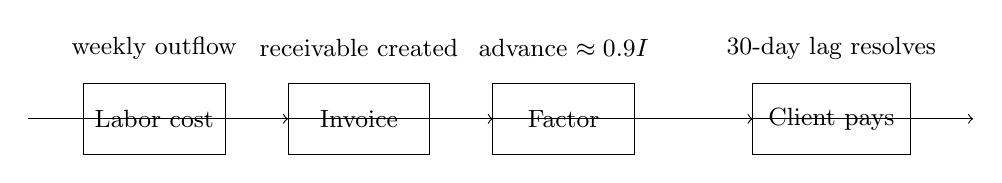
\begin{tikzpicture}[x=1cm,y=1cm]
\draw[->] (0,0) -- (12,0);
\draw (0.7,-0.45) rectangle (2.5,0.45);
\node at (1.6,0) {\small Labor cost};

\draw (3.3,-0.45) rectangle (5.1,0.45);
\node at (4.2,0) {\small Invoice};

\draw (5.9,-0.45) rectangle (7.7,0.45);
\node at (6.8,0) {\small Factor};

\draw (9.2,-0.45) rectangle (11.2,0.45);
\node at (10.2,0) {\small Client pays};

\draw[->] (2.5,0) -- (3.3,0);
\draw[->] (5.1,0) -- (5.9,0);
\draw[->] (7.7,0) -- (9.2,0);

\node at (1.6,0.9) {\small weekly outflow};
\node at (4.2,0.9) {\small receivable created};
\node at (6.8,0.9) {\small advance \(\approx 0.9I\)};
\node at (10.2,0.9) {\small 30-day lag resolves};
\end{tikzpicture}
\caption{Transcript-derived cash-cycle sketch. Weekly expense leaves first, a receivable is created, factoring advances cash against the invoice, and the client payment arrives only after the lag.}
\end{figure}

\section{From Revenue to Replication}

Once the capital problem is on the table, the lecture asks the next natural question: how does one move from a smaller business toward a much larger one? Louis's answer is structured, and we should preserve that structure.

The first piece is customer-centered growth. He describes a consultative sales approach: do not merely sell labor; show the customer that the arrangement makes the customer's business more profitable and more competitive. The business grows not simply by closing transactions but by taking over more and more of the customer's operating burden.

The second piece is internal capital. The lecture is explicit: growth requires both demand and money. We can encode the bottleneck schematically as
\begin{equation}
G \le \min\{D,K\},
\end{equation}
where \(D\) is signed customer demand, \(K\) is fundable delivery capacity, and \(G\) is realized growth. If customers exist but the firm cannot finance execution, growth stalls. If cash is available but there is no customer demand, the same is true.

The third piece is operational consistency. Once new sites are won, the company needs procedures, training, and repeatable execution. The interview uses the language of standard operating procedures and daily operating discipline. The chapter should preserve this ordering: first customers, then funding, then replication.

But the lecture does not stop there. It then makes a sharper organizational claim. A company cannot scale if accountability is imposed without corresponding authority. People who are held responsible must also be empowered to act, to think, to push, and even to contradict the founder.

\paragraph{Three layers of scale.}
In the lecture's logic, organizational scale requires all three of the following:
\begin{itemize}
\item customer value, so that business continues to flow in;
\item balance-sheet strength, so that the new business can be financed;
\item distributed authority, so that execution improves instead of bottlenecking at the top.
\end{itemize}

This is one of the deepest moments in the lecture. Louis would rather sit in a room where other capable people tell him where he is wrong than build a firm whose intelligence never exceeds the founder's own perspective. The notes should preserve that point, because it is the organizational analog of the earlier financial argument. Just as revenue must not be extracted too early, judgment must not be centralized too completely.

\section{Relationships, Credit, and Long-Term Negotiation}

At this point the interview is briefly interrupted by a promotional segment. We set that aside and return where the argument resumes: relationships.

The first relationship class is with bankers. The lecture revisits the earlier factoring story, but now from a more mature perspective. Invoice factoring was not the destination. It was a bridge toward conventional credit. Even before the balance sheet was strong enough, Louis began building relationships with bankers, learning from them what the balance sheet had to look like, and then demonstrating that he could move the company in that direction.

The result, eventually, was a traditional line of credit large enough to change the business permanently. The numbers remain striking. By roughly the third year, the borrowing need was on the order of \$14 million. The company was still young, but credibility, discipline, and repeated execution had turned the firm's narrative from speculative story into bankable pattern.

The second relationship class is lateral rather than vertical: peer groups. Louis's regret is not that he lacked enough sales breakfasts or enough weak networking. His regret is that he did not enter earlier into groups where owners could exchange actual operating experience, compare failures, and save each other from needless time loss. The lecture's point is very precise. Shared experience is a form of capital.

The final movement concerns negotiation. Here again the lecture refuses a short-term frame. If a procurement department is obsessed with price today, Louis suggests not necessarily fighting on that single axis. Let the buyer have the superficial win if necessary, but redesign the structure so that compensation rises with measurable results.

In a schematic notation we may write
\begin{equation}
P_{\mathrm{deal}} = P_0 + \beta S,
\end{equation}
where \(P_0\) is the base price and \(S\) is some verified savings or measurable result delivered to the client. Another version, closer to the lecture's emphasis on client performance, is
\begin{equation}
\Delta P = \gamma\,\Delta \Pi_{\mathrm{client}},
\end{equation}
where \(\Delta \Pi_{\mathrm{client}}\) is the improvement in client profit or bottom-line performance attributable to the relationship.

These are not formulas quoted by the speaker. They are compact ways of stating the lecture's logic. Do not argue only about today's margin. Tie compensation to future results. If the service truly makes the client's business better, then higher pay on the back end is no longer a speculative ask; it is a share in created value.

This returns us, beautifully, to the lecture's recurring theme. A relationship-centered business is not the opposite of rigorous business. It is rigorous business extended across time.

\section{Summary}

The lecture begins with luxury and ends with structure. Between those two points it develops a coherent operating philosophy: delegation multiplies capacity, restraint protects optionality, early capital should be treated with suspicion when it comes bundled with control loss, working capital is often the real technical problem behind growth, retained earnings build freedom, and leadership requires distributed authority.

The arithmetic in the lecture is approximate, but the architecture is sharp. First create proof of concept. Then solve the cash-cycle problem without destroying ownership if you can avoid it. Then convert discipline into balance-sheet strength. Then build a company whose procedures, people, and relationships allow it to think and act beyond the founder. That, in these notes, is the hidden machine underneath the visible life.